\chapter{Project Management}

\section{Project planning}
\begin{figure}[H]
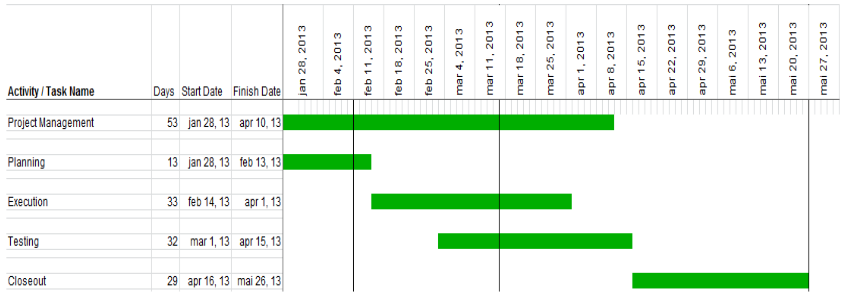
\includegraphics[scale=0.8]{images/gantt-diagram.png}
\caption{Gantt diagram. Milestones are marked using vertical lines}
\end{figure}

\section{Development method}
Iterative model based on lean with proposal to the customer weekly. This agile methodology decreased the project risk and secured a complete and functional system for the customer. The customer could then influence our work and adjust potential misconceptions early in the project. Prototypes and demonstration for SINTEF were made in the beginning to validate the understanding of the requirements.

\section{Team roles}
The group was organized in different roles based on skill and experience. Each team member was given a responsibility for some code-packages. Further, the team was divided in six subgroups where each subgroup had one responsible leader. These were respectively group leader, documentation and substitute leader, Android and GUI, arduino and PUI, over the air and test leader. The group worked in three subgroups of two, which made it easy to do pair-programming and individual work.

\subsection{Role evaluation}
The division of the group was an important feature. Every member knew who to contact about a specific problem, and who to contact regarding different tasks.\\

\begin{description}
	\item[Group leader]{was responsible the progress in the overall project. This person ensured progress and priorities for deadlines.}
	\item[Documentation and subsitute leader]{was responsible for management of documentation and reports. In absence of the group leader, this person took on the group leaders responsibilities. This person were also responsible for contact with the customer and supervisor.}
	\item[Android and GUI]{was responsible for the arduino part of the project. This implies contacting the arduino-lab, requirements of hardware and the coding part. This role were also responsible for development of the PUI examples.}
	\item[Arduino and PUI]{was responsible for the arduino part of the project. This implies contacting the arduino-lab, requirements of hardware, the coding part and over-the-air installation. This role were also responsible for development of the PUI examples.}
	\item[Over the air leader]{was responsible for programming the arduino over the air. This person was responsible for making the first prototype with a bluetooth connection.}
	\item[Test leader]{was responsible for developing and executing tests for the complete project.}
\end{description}

\begin{table}
\begin{tabular}{|l|l|}
\hline
	{\bf Name} & {\bf Role}\\
\hline
	Jeppe Benterud Eriksen & Group leader\\
\hline
	Nina Margrethe Smørsgård & Documantation and subsititue leader\\
\hline
	Robin Tordly & Android and GUI leader\\
\hline
	Bjørn Arve Fossum & Arduino and PUI leader\\
\hline
	Ståle Semb Hauknes & Over the air leader\\
\hline
	Wilhelm Walberg Schive & Test Leader\\
\hline
\end{tabular}
\caption{Roles}
\end{table}

\section{Communication}
Most of the communication within the group was done at group meetings and when the group were working together. For communication between group members outside the meetings it was decided that the group should only use email and Skype. This was decided to avoid the confusion that might arise from using numerous channels of communication. Mobile phone was also used when immediate contact was necessary.\\
\newline
Communication between the group and the customer were mainly done in meetings or by email. The same applies for communication with the supervisor.

\section{Risk analysis}
\captionof{table}{Risk analysis}
\label{fig:risktable}
\begin{longtable}{|m{0.15 \textwidth}|m{0.1 \textwidth}|m{0.1 \textwidth}|m{0.1 \textwidth}|m{0.185 \textwidth}|m{0.185 \textwidth}|}
\hline
	\rowcolor{Gray}
	\textbf{Description} & \textbf{Likeli{-}hood} & \textbf{Impact} & \textbf{Impor{-}tance} & \textbf{Preventive\newline Action} & \textbf{Remedial\newline Action}\\
	\endfirsthead%
	\multicolumn{6}{l}%
	{{\bfseries Continued from previous page}} \\ \hline
	\rowcolor{Gray}
	\textbf{Description} & \textbf{Likeli{-}hood} & \textbf{Impact} & \textbf{Impor{-}tance} & \textbf{Preventive\newline Action} & \textbf{Remedial\newline Action}\\
\hline
	\endhead%
	\hline

	\hline \multicolumn{6}{|l|}{{Continued on next page}} \\ \hline
	\endfoot%

	\endlastfoot%

	Illness & 7 & 2 & 14 & Good\newline communication and effective use of GitHub & Increase workhours and exchange tasks and\newline responsibilities\\
\hline
	Project\newline complexity & 6 & 5 & 30 & Don't take on too much work & Cut down the demands\\
\hline
	Customer\newline issues & 1 & 5 & 5 & Agreement with customer and weekly feedback from customer & Use the\newline original\newline requirement specification\\
\hline
	License\newline incompability & 7 & 7 & 49 & Avoid\newline integrating components with incopatible licenses & Discover other implementations or implment from scratch\\
\hline
	Group\newline conflicts or disagreements & 3 & 3 & 9 & Keep close\newline contact to avoid\newline surprises.\newline Leader takes\newline action & Contact\newline supervisor and make an\newline appointment\\
\hline
	Over the air complexity & 8 & 8 & 64 & Have multiple\newline alternative\newline solutions and keep close\newline contact with customer & Detail what was attempted as well as why it couldn't be solved in the final report.\\
\hline
	Personal matters & 8 & 5 & 40 & Not much\newline preventative action can be taken & Keep in touch and stay\newline updated. In case you still can do tasks, claim one and tell the\newline others\\
\hline
\end{longtable}